\section{Flight Controller}

\subsection{Initial plan and concept changes}
The main objective of this bachelor thesis is to build a small variable pitch quadrotor, which will be used to measure the response time and compare it with a fixed pitch quadrotor to determine the effects it has on stability. The plan was initially to change the Pixhawk flight controller, to get it to work with radio control and the Pixhawk autopilot. However, integrating Pixhawk autopilot is not trivial, especially to get it to work with the variable pitch quadrotor. It requires a significant change of a quite large flight controller, consisting of hundreds of thousands of lines of code. 
\\\\
The approach was altered early, after a discussion with FFI, based upon all of the changes that would have to be made in the flight controller. Not to speak of all the hours needed to understand the flight controller at a decent level. 
\\\\
With access to Kongsberg Innovation Center, containing a high motion capture system (Qualisys), the team decided to build a flight controller from scratch. The plan was to use the Qualisys system to track the quadrotor and give data about its position. Using the high motion capture system also gave us the possibility to make the quadrotor autonomous. The disadvantage with this choice is the limitation with access to the lab under development. This also forces any further use to be at a facility containing Qualisys or a similar high motion capture system. This means that for FFI to be able to use this system, they would need a high motion capture system. Even with these two major disadvantages in consideration the team decided that it was worth using this facility to get accurate and repeatable data.  
\\\\
The initial thoughts was to use an external computer connected to the high motion capture camera as a flight controller.\\
\begin{figure}[H]
          \centering
            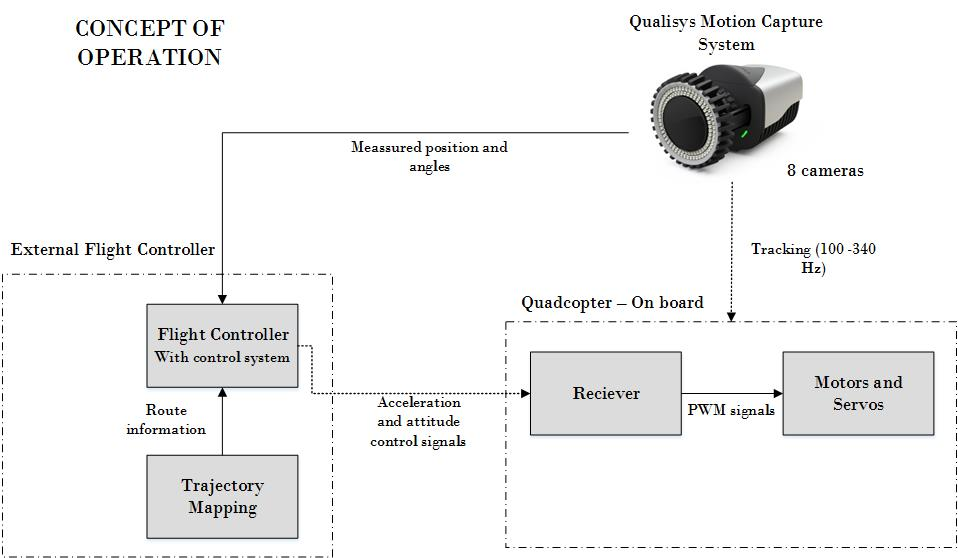
\includegraphics[scale = 0.6]{VAPIQ-PICTURES/ConceptOfOperation.jpg}
                \caption{Original Concept of Operation}
                \label{OCO}
            \label{dir}
\end{figure} 
\newpage
\noindent 
In this concept the plan was to use the information received from QTM to do calculations on an external computer. The initial assumption was that this would give an advantage when writing our own flight controller software. Advantages with computing externally are increased computational power and less hardware such as sensors on the quadcopter. 
\\\\
QTM provides six different values (x, y, z, $ \phi, $ $ \theta $ and $ \psi $). The goal is to keep the quadrotor stable and agile in air. The plan was taking the information provided about its position and rotation and compute algorithms to determine roll, pitch, yaw, and thrust change for each motor. The computed data would then be sent back to the quadrotor wirelessly with simple motor and servo signals for it to execute. This was supposed to run in a loop and update at a rate of minimum 50Hz. Getting an update every 20ms. The external PC would need to gather information, compute and send it back to the quadcopter. \\
\\
However testing showed that the latency would be too high. The project would not work or at best heavily restrict agile maneuvering. The communication part took longer time than expected. The bluetooth signals alone used about 0.08s giving an update frequency of 12.5Hz, provided that the computation and Qualisys sampling happens instantly. The combination of the time it would take for Qualisys to update the computer and the computer to send the signal to the quadcopter was more than 20ms. An update frequency of 12.5Hz or lower would limit the agility of the quadrotor. After analysing this concept it became clear that improvements was needed.

\begin{figure}[H]
          \centering
            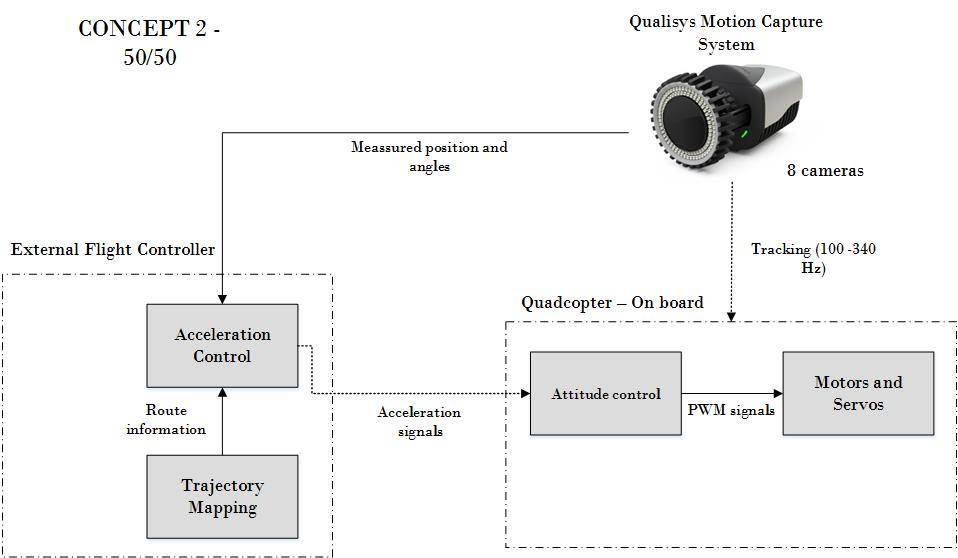
\includegraphics[scale = 0.67]{VAPIQ-PICTURES/Concept2.jpg}
                \caption{Concept 2}
                \label{Con1}
            \label{dir}
\end{figure} 
\newpage
\noindent
The second concept proposed for the flight controller (see Fig. \ref{Con1}) consist of moving the control algorithm to the quadrotor. The control feedback pace would improve by moving the control algorithm, adding an IMU and a processing unit to the quadrotor. The control feedback will only need to sample data from the IMU, compute the desired change on-board and update the motors. 
\\\\
The external computer still control the acceleration control and trajectory mapping. This keeps the advantage of using Qualisys, mapping a route for reliable and reproducible data and more computational power. This concept has, unlike the first concept, a fast control loop as well as not getting drift over time. 
\begin{figure}[H]
          \centering
            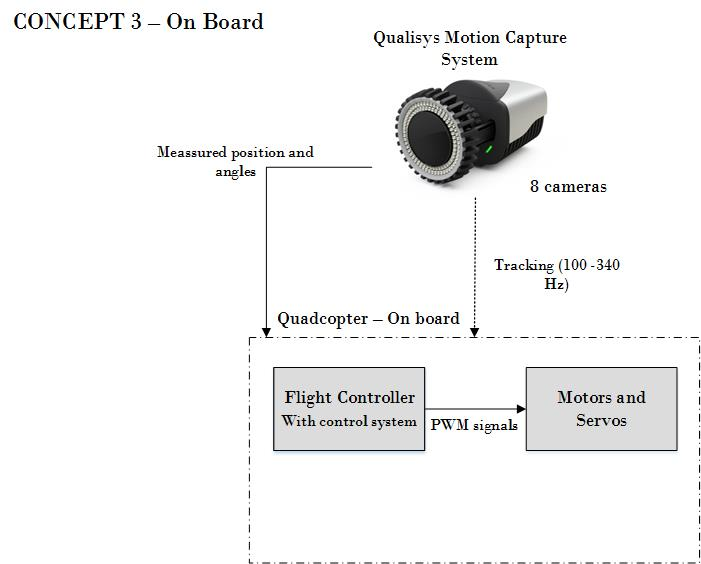
\includegraphics[scale = 0.67]{VAPIQ-PICTURES/Concept3.jpg}
                \caption{Concept 3}
                \label{Con2}
            \label{dir}
\end{figure} 
\noindent
Another concept is to move all of the code to the quadrotor. Moving the control algorithm and the attitude control loop to the quadrotor will improve the attitude control feedback and limit the delay for the overall movement. The downside with this concept is that it requires more computation time and/or computation-power. 
\\\\
In this concept Qualisys could be moved and a radio controller could be used instead. This would be a far easier task to complete. Instead of making an autonomous quadrotor. Qualisys would only be an observer, and the data produced is dependent on the user. Fig. \ref{Con2} shows Qualisys only as an observer. If we choose to still use Qualisys it would be difficult to change the course, and all movement would need to be pre-programmed into the quadrotor code. The quadrotor can use Qualisys to avoid drift over time that would otherwise happen, if it only where to fly based upon it's assumed position. The sensor readings would change over time and provide a certain bias. 

\begin{figure}[H]
          \centering
            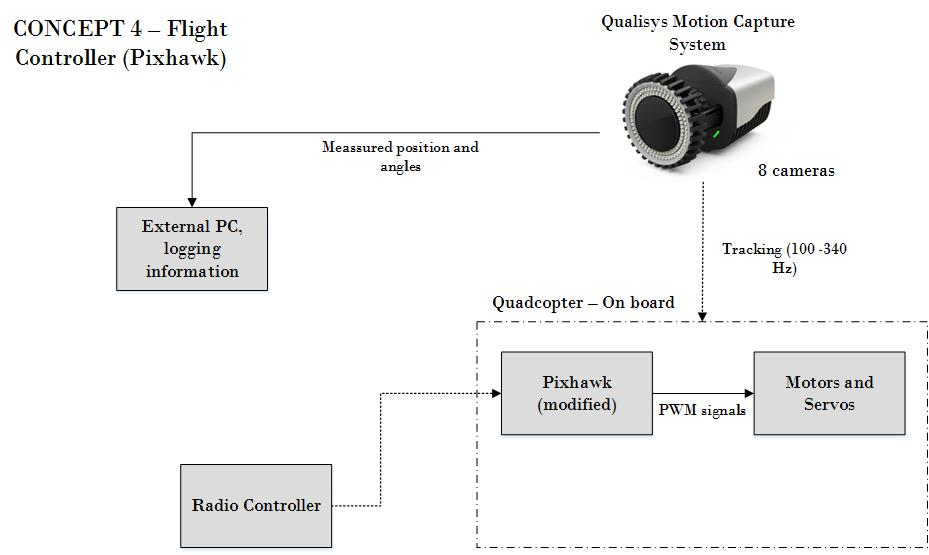
\includegraphics[scale = 0.67]{VAPIQ-PICTURES/Concept4.jpg}
                \caption{Concept 4}
                \label{Con3}
            \label{dir}
\end{figure} 

\noindent The fourth concept is to go back to the original plan to modify a Pixhawk. Qualisys can be used as an observer and run the system with a radio controller. This is probably the easiest option to get a flying variable pitch quadrotor helicopter. In theory it should be possible to achieve variable pitch flight by changing the thrust relative to the pitch, and change the thrust input with the propeller pitch. Nevertheless we would have the same problem as in concept 2, where it would be difficult to get valuable scientific data. The other option is to integrate the Pixhawk flight controller with the Qualisys system. 
\\\\
The current assumption is that implementing Qualisys into the Pixhawk autopilot and changing the required part in the code would take a substantial amount of time. A possible solution would be to modify it to work with radio controller and then expand it to get signals from a computer in order for it to work autonomously. Radio control can be desired because of the implementation time is likely to be shorter.

\subsubsection{Current Concept \& Analysis}
The original concept was very promising in the way it would give us accurate scientific data, needing less hardware on the quadrotor, and more computation power. This concept has one disadvantage related to the latency in the overall system. The quadrotor needs to correct for changes quick and a too high latency limits the system. To correct for this the concepts was created, each providing their advantages and disadvantages. 
\\\\
Both concept two (Fig. \ref{Con1}) and three (Fig. \ref{Con2}) removes this latency by adding an IMU that can sample at 1KHz for the accelerometer data and 8KHz for the gyro data. This gives us an update frequency of 50Hz, compared to 12.5Hz by using Qualisys, given 20 samples to filter vibrations and spikes. However this requires more hardware on the quadrotor making the quadrotor heavier. For the concept with the on-board and off-board flight controller, see Fig. \ref{Con1}, it involves more communication between the systems. The deciding factor, in our case, between these two concepts is that the user will have more control over the quadrotor. For the 50/50 concept the user can send signals to python in real-time, to change its trajectory. This is harder to do with the quadrotor flight controller. Normally this would be controlled with a radio controller and not a pre-programmed route. 
\\\\
The two remaining concepts, see Fig. \ref{Con1} \& Fig. \ref{Con3}, is making a 50/50 version or modifying the pixhawk. This was for us a difficult choice, considering our knowledge gaps in both these areas. It is possible to modify the pixhawk code, an already existing flight controller. Which is optimized for fixed pitch quadrotors. The pixhawk however is quite large and could be harder to modify and integrate with the motion caption system. On the other side it would be easier to integrate the motion caption system in a self-developed code. The problem is that the self-developed code would not be optimized for neither fixed nor variable pitch. The time it takes to optimized is also quite long.
\\\\
After taking these advantages and disadvantages from each concept and analysing them, the team came to the conclusion that going for concept two was the best for our case, see Fig. \ref{Con1}. 

\subsection{On Board}
The on-board flight controller mainly consist of the inner control loop. This is the loop that helps the quadrotor keep steady. Its only objective is to achieve  stabilisation of the quadcopter in a given rotation provided by the external system. It uses multiple libraries like Servo.h for sending and SoftwareSerial.h for communication. It expects to receive the angles the quadcopter should keep to get to a given position, or to stay at it is current. It also expects to receive the amount of thrust it needs to stay at the same altitude. 

\subsubsection{Calibration, arming and sensor readings}
The first thing the quadcopter does when turned on, is to calibrate the sensor. It takes 1000 samples of the current location and calculates offset. This was a great help when implemented and changed angle and angular velocity start error by $\pm$ 10 deg/(deg/s) to $\pm$ 0.04. Calibrating the 9250 MPU sensor improved the accuracy of the readings by a factor of 250. The quadrotor has to be in zero degrees when starting, else the calibration will not work. Another disadvantage is that the quadrotor is quite vulnerable in the calibration process. Any disturbance at that time will mess with the sensor data offset.
\\\\
When the quadrotor is calibrated a light is lit to mark this. Making it easier for the user to register this. The quadrotor then waits for a bluetooth signal matching its starting protocol. When this signal is received the quadrotor will arm the motors by sending PWM signals to each motor (1000$\mu$s). And waiting three seconds for the motors to be ready. 
\\\\
The Quadrotor then enters the control loop. The control loop consists of sensor readings, the control system and sending PWM signals. The first thing the code does is to check if it has been sent a bluetooth signal to turn it off. If no off signal has been sent, then PWM (1000$\mu$s) signals are sent to each motor. If such a signal is received it breaks out of the inner-loop and waits for a new starting signal. If no such signal is sent, then it reads the gyro and accelerometer data. This data gets converted to degrees and then goes through a lowpass filter and a weighted moving average filter. This is to remove some of the vibration noise created by the propellers. 
\\\\
The filtered data then gets saved to an array, and it rinse and repeat until it has taken a given amount of samples (currently set to five samples, this will however change soon). \\
\newpage
\subsubsection{Control System}
When the quadrotor has calibrated, armed and have multiple sensor readings, the control system starts. A block diagram of the control system is provided in Fig. \ref{fig:dir}.
\begin{figure}[H]
          \centering
            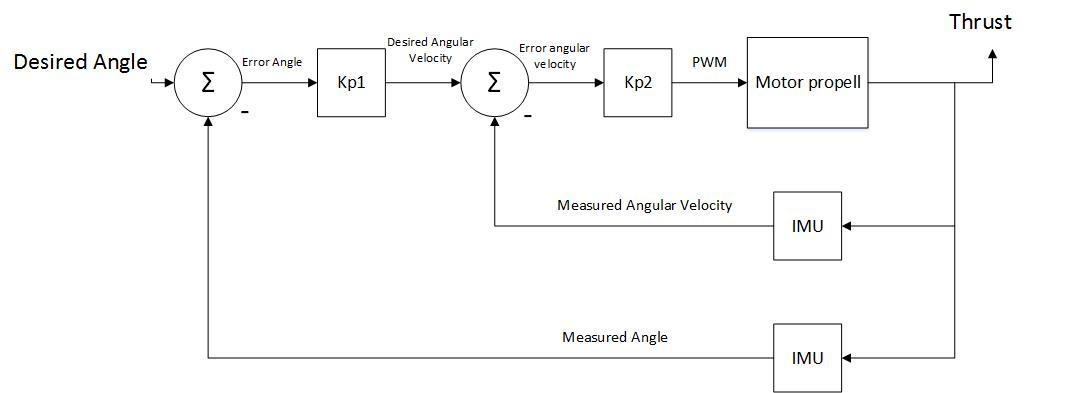
\includegraphics[scale = 0.62]{VAPIQ-PICTURES/CSBD.jpg}
                \caption{Control System}
                \label{CSBD}
            \label{fig:dir}
\end{figure} 
\noindent
It first calculate the average of the sample data for angle and angular velocity. The angle error is calculated by taking the desired angle and subtracting the actual angle. 
\begin{equation}
   Angle Error = Desired Angle - Measured Angle
\end{equation}
\noindent
By taking the error of the angle and multiplying it with a constant the result will be the desired change in angular velocity. This is given that the constant is tuned properly.
\begin{equation}
   Desired Angular Velocity = Angle Error * Kp
\end{equation}
\noindent
The bigger the error the larger the speed the quadcopter wants to gain. The closer the quadcopter are to the goal, the slower it want to move, so multiplying with a constant here can give us this. Taking this desired angular velocity and subtracting from the actual, gives us the angular velocity change the quadcopter want to make.
\begin{equation}
   Angular Velocity Error = Desired Angular Velocity - Measured Velocity
\end{equation}
\noindent
The error in angular velocity can be used as the difference the quadcopter want each motor to give, by multiplying this value with another constant. This number can give us the differential of force the quadcopter want to make for each motor. \\
\begin{equation}
   dThrust =   Angular Velocity Error * Kp2
\end{equation}
\noindent

\begin{figure}[H]
          \centering
            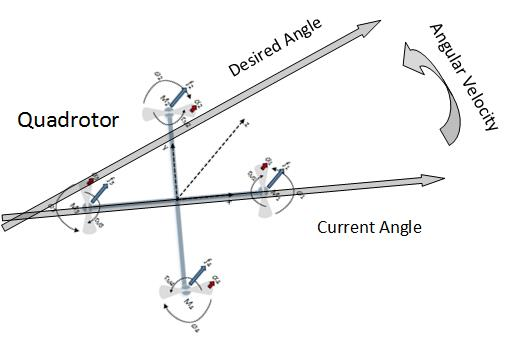
\includegraphics[scale = 0.67]{VAPIQ-PICTURES/OnBCS.jpg}
                \caption{Stability Control}
                \label{StabiilityControl}
            \label{dir}
\end{figure} 
\noindent
Doing this for both motor 1 and motor 3, and motor 2 and motor 4. To give an specific example if the differential thrust is 20$\mu$s and the thrust needed for hover is 1300$\mu$s: 
\\\\
$$motor1 = Hover (1300) + differential (20)$$ \\
$$motor3 = Hover (1300) - differential (20)$$ 
\\\\
If the differential thrust is negative, motor 3 will increase and motor 1 will decrease. The PWM signals varies from 1000$\mu$s to 2000$\mu$s. Then the given force for each motor is sent as a PWM signal, and the control loops rinse and repeat.
\\\\
This type of controller is a proportional-integral-derivative controller (PID controller). Although a P controller is implemented at this moment, but a PD controller will be added in the future versions of the controller. This controller uses feedback to calculate an error between a desired setpoint and the actual variable measured by a sensor. In this case a angle and the angular velocity measured by the IMU.

\subsection{Communication}
A HC-06 bluetooth device are used in this project, which are connected to the on-board arduino. Using a Xbee wi-fi module was considered, but we ended up on the conclusion that the bluetooth device would be sufficient. It is used as a slave and needs to be connected from the computer with a physical address. The software serial library helps when connecting to both the serial and bluetooth cable at the same time. Information is sent by using a string that contains the angles and thrust. The string gets interpreted when it reaches the arduino and is casted to integer.
\\\\
The external computer can get information from Qualisys by calling some software functions. First calling the qt.setup() function to setup the connection, and then call on qt.getAttitude() to get the position and rotation. We've however struggled some on getting the most recent information. Further testing is required. 

\subsection{Off Board}
The off board flight controller deals with the information provided from Qualisys and finding the path. It can decide the pitch and roll angle to the quadrotor. The quadrotor on-board code then works to keep it stable with the given pitch and roll. It also controls the thrust. Making sure the quadrotor is in the right altitude, and correcting for errors. 
\\\\
The main goal with the off-board controller is to decide the path of the quadrotor in flight, and provide it with information required. 
\subsubsection{Establishing Connection}
The off-board code first tries to establish connection with Qualisys. If no contact is achieved it will not start. When contact is achieved it will send a start signal to the quadrotor, which in return will send a signal back when the motors are armed. When both contact with Qualisys and the quadrotor is achieved the program will start computing. \\
\subsubsection{Off-Board Control System}
The off-board control system computes the angles and desired position, and sends this information to the quadrotor. The quadrotor start by storing the start position and the current time. \\
The external computer then gets the new position and rotation of the quadrotor. If no data is received a counter is increased, and the last position and rotation measured is the current. If this happens five times the quadrotor will stabilize and land. If the contact is received the counter resets. \\
When the off-board gets the information from Qualisys it calculates the current velocity of the quadrotor. The last position and time is updated as the current time and position. \\
\\

\begin{figure}[H]
          \centering
            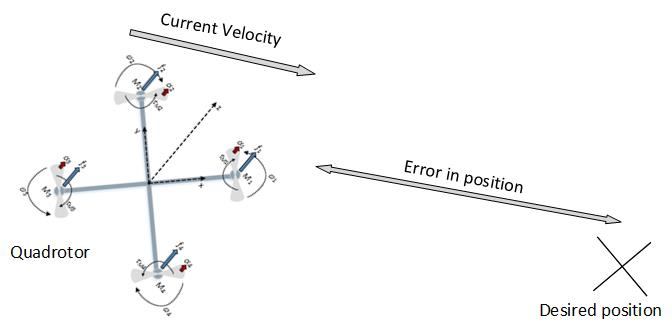
\includegraphics[scale = 0.67]{VAPIQ-PICTURES/OBCS.jpg}
                \caption{Trajectory Control}
                \label{TrajectoryControl}
            \label{dir}
\end{figure} 
\noindent
The next steps in this algorithm is very similar to how the quadrotor keeps steady. The first step is finding out the error in position. This is done by taking the desired position and subtracting the current. 
\begin{equation}
   Error Position = Desired Position - Measured Position
\end{equation}
\noindent
Multiplying the desired position with a constant can give us a value for the desired speed. 
\begin{equation}
   Desired Velocity = Error Position * Kp
\end{equation}
\noindent
The desired speed will then change regarding to the distance, the further away from the desired position, the bigger roll and pitch angle is desired. The error between the desired speed is then found by subtracting from the current speed.
\begin{equation}
    Error Velocity = Desired Velocity - Measured Velocity
\end{equation}
\noindent
This error in speed can be directly applied to the roll and pitch angle when multiplied with another constant. 
\begin{equation}
   dAngle =  Error Velocity * Kp2
\end{equation}
\noindent
The thrust also gets computed in this algorithm, the force for the pitch and the force for roll and dividing by their respective angles. The total sum is then added together as well as added with the sum of the error in Z-position multiplied with a constant. 
\begin{equation}
        ThrustX = \frac{thrust}{cos(angularX)}
\end{equation}
\noindent
\begin{equation}
        ThrustY = \frac{thrust}{cos(angularY)}
\end{equation}
\noindent
\begin{equation}
        Thrust = \frac{thrustX + thrustY}{2}  + errorZ*kpZ
\end{equation}
\noindent
Then the values computed only need to be limited, in order to not change the roll and pitch to an angle we can't keep in the same altitude. All the data computed in the algorithm then gets sent to the quadrotor and the code rinse and repeat until it is stopped.

\subsection{Qualisys}
In this project the Qualisys Tracking Manager(QTM) system is being utilized and this chapter explains what it is, how it works and why we are using it in this project. \\
\\
Qualisys is a Swedish motion capture system. The company have developed multiple camera types and software which are able to capture real-time motion of fast moving objects with great precision. Qualisys have features such as capturing 2D, 3D and 6DOF data in real time with low latency. The system tracks small spherical markers placed on the object that will be tracked. The data will be logged and can be analysed. It is used in Medical, Engineering, Sport and research applications, such as quadcopters and VR projects \cite{QTM}.

\begin{figure}[h]
          \centering
            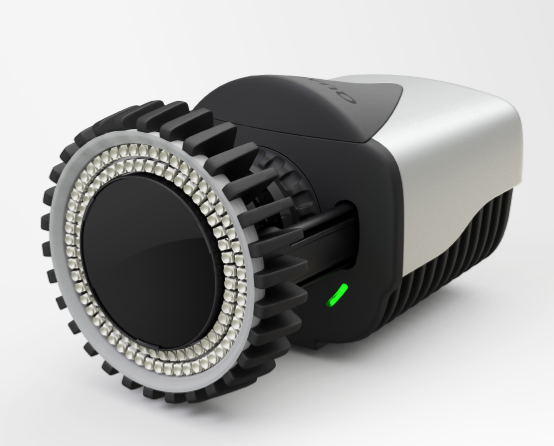
\includegraphics[scale = 0.33]{VAPIQ-PICTURES/m3.png}
                \caption{Miqus 3}
                \label{m3}
            \label{dir}
\end{figure}

\subsubsection{How does it work}
When you want to track an object, you can add spherical markers on the object, in our case a quadcopter. These spherical markers can vary in size from 19mm to 6.5mm. When the quadcopter move the position and rotation it will be tracked. \\
\begin{figure}[h]
          \centering
            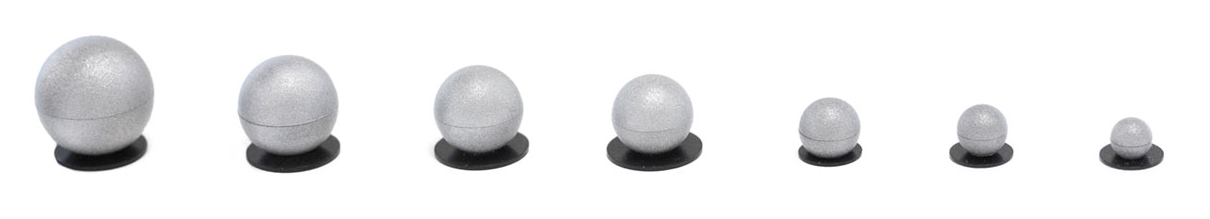
\includegraphics[scale = 0.35]{VAPIQ-PICTURES/sphere.png}
                \caption{Spherical markers to QTM}
                \label{sphere}
            \label{dir}
\end{figure}
\\
The input Qualisys needs is the spherical markers and it needs three markers in the same z-plane. This can give information about where it is and what’s the front (one marker) and what’s the back (two markers). It also needs another marker to be able to detect what’s up and what’s down on the quadcopter. 
\\\\
This information is then sent on Wi-Fi to an external computer and can be displayed in the Qualisys Tracking Manager. The QTM is a GUI which displays the output from the cameras. The output given by Qualisys is the position of the quadcopter (the x, y and z coordinates) and It is rotation ($ \phi,$ $ \theta $ and $ \psi $). This information is displayed in the GUI giving a visualisation of the position of the quadcopter. The GUI shows one coordinate system related to the room, and another coordinate system related to the body of the quadcopter.
\begin{figure}[ht]
          \centering
            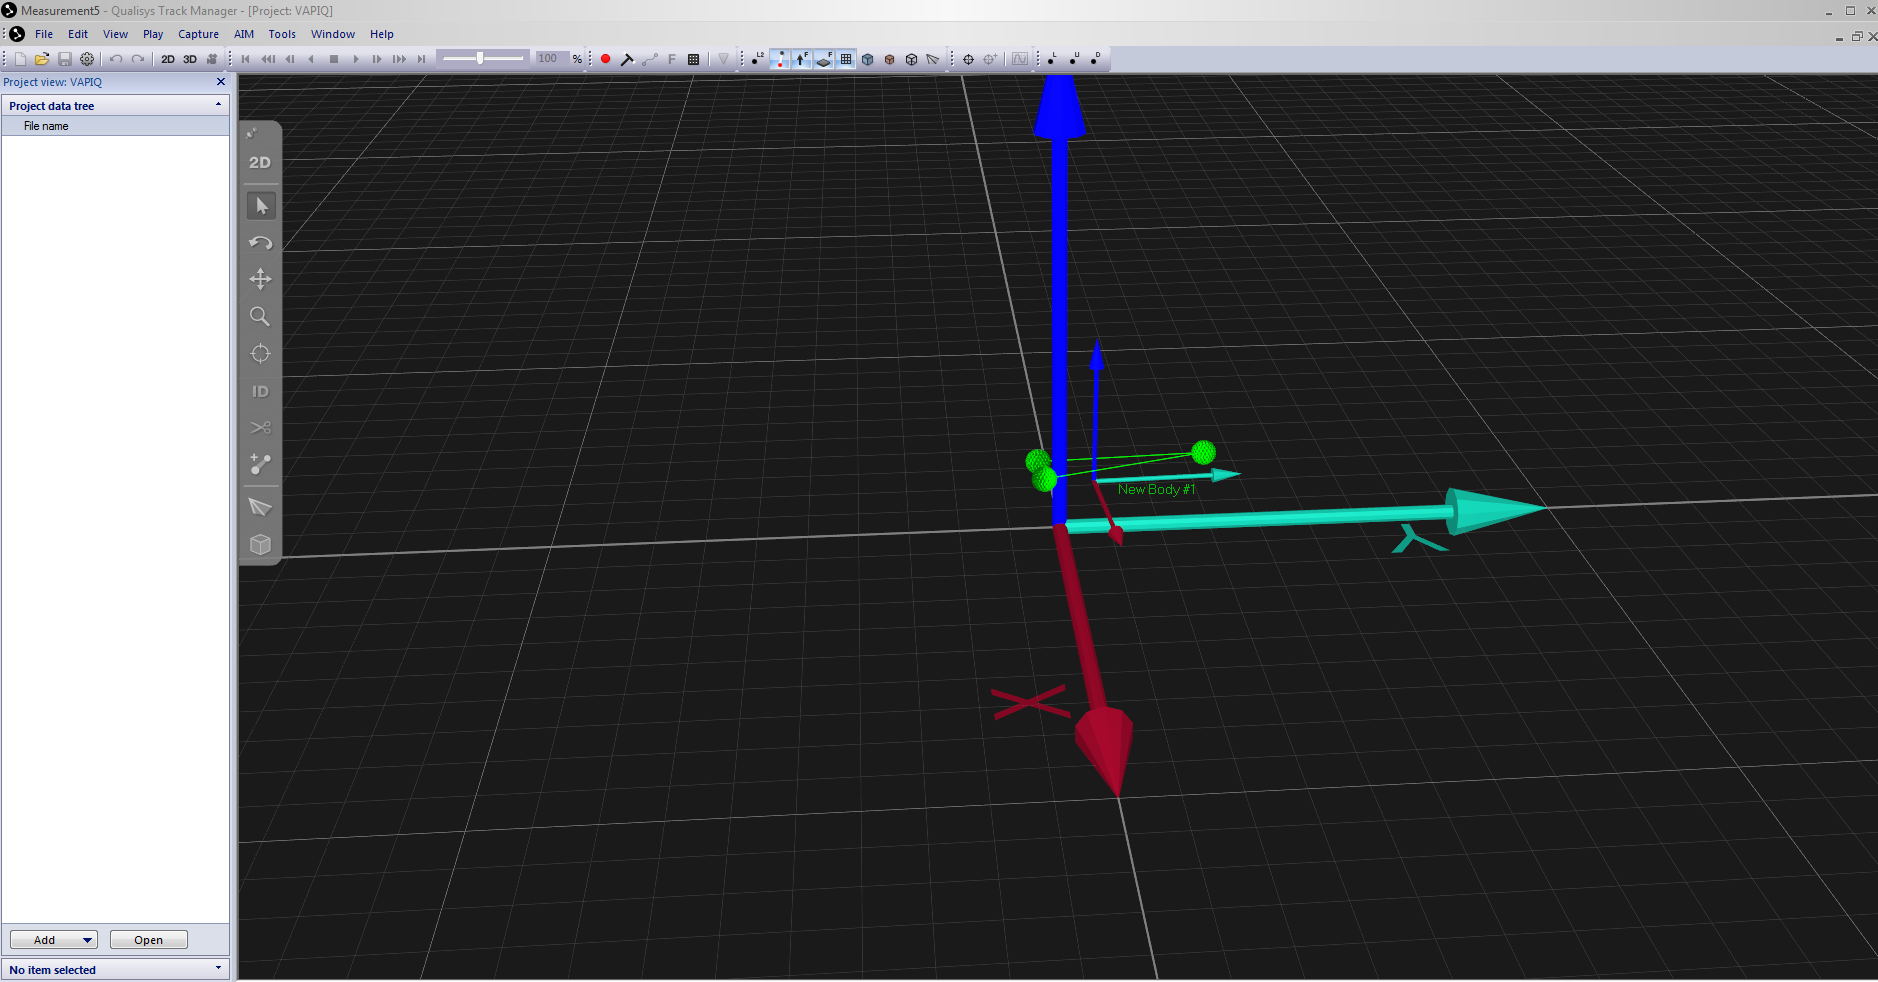
\includegraphics[scale = 0.25]{VAPIQ-PICTURES/qtm.png}
                \caption{Qualisys Tracking Manager 3D}
                \label{qtm3d}
            \label{dir}
\end{figure}
\noindent However, to get the coordinate system of the quadcopter you would need to configure the body, which is done before any testing can take place. This is done by removing potential noise and confirming which marks the body will consist of. 
\\\\
The AIM model (automatic identification of markers) can be added to any measurement and captures similar motions compared to the model. When the model is identified in real-time the tracker tracks it with frame rate independent performance. The GUI helps with visualization and can ease testing. We can detect the route of the quadcopter in real-time or save the route to replay it for a more detailed study afterwards.  The Miqus3 camera can detect the position and rotation up to 340 times per second. \\\\
\begin{figure}[h]
          \centering
            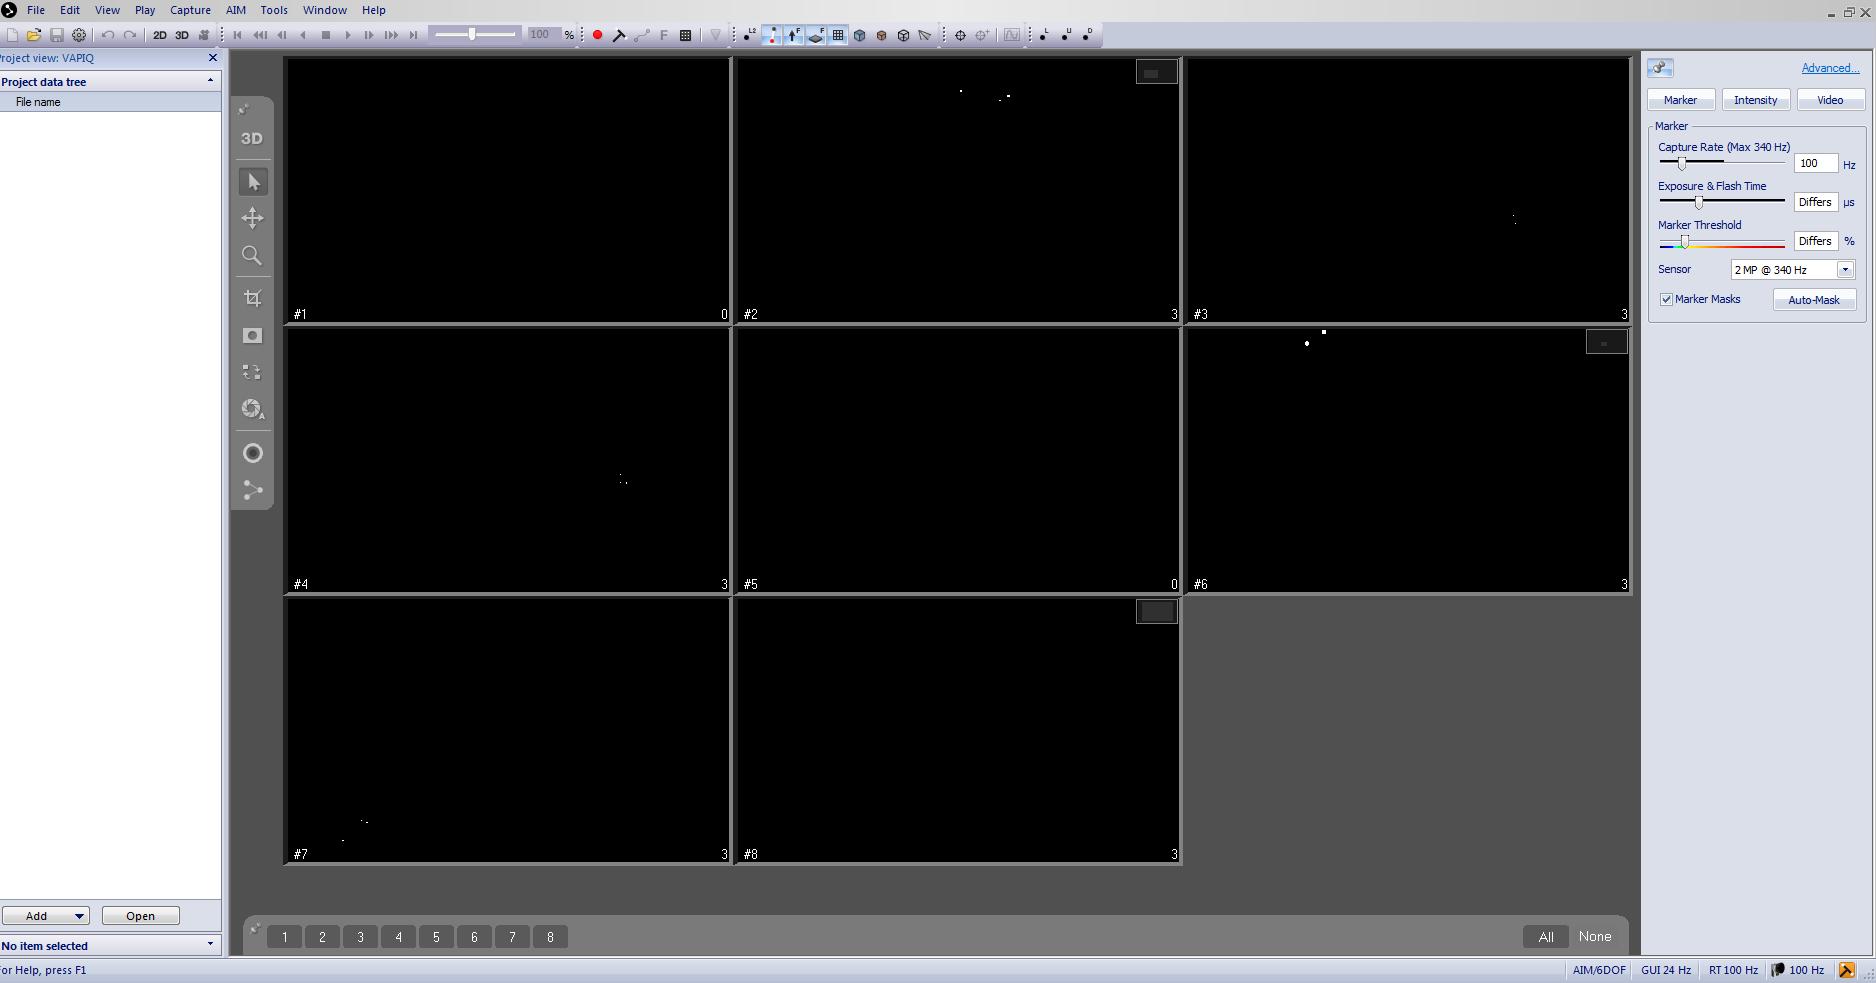
\includegraphics[scale = 0.25]{VAPIQ-PICTURES/qtm2d.png}
                \caption{Qualisys Tracking Manager 2D}
                \label{qtm2d}
            \label{dir}
\end{figure}
\\\\
\begin{figure}[h]
     \begin{minipage}[t]{0.45\textwidth}
    \textbf{Key features:}
        \begin{itemize}
            \item Optical real-time tracking
            \item Recordable
            \item Tracking in 2D, 3D and 6DOF
            \item Update frequency up to 340Hz
        \end{itemize}
     \end{minipage}
        \hfill
    \begin{minipage}[t]{0.45\textwidth}
        \textbf{System details:}
        \begin{itemize}
            \item Runs with Windows
            \item Wireless LAN option
            \item Compatible with matlab and avi 
            \item Single cable from cameras to computer
        \end{itemize}
    \end{minipage}
\end{figure}

\vspace*{0.03cm}
\subsubsection{Why did we choose Qualisys?}
The main objective of our project is to compare a variable pitch quadcopter with a fixed pitch quadcopter. The way we have chosen to do this is with a tracking system. The tracking system will provide relevant data both for testing and research. It will provide reproducible research data and will make it easier when testing for errors. The best available track system for us is at Kongsberg Innovation Center (KIC). They have a lab available with eight Qualisys cameras. \\
\\
Using this system will lead to advantage in body weight of the quadrotor. Most of the equipment needed on a quadcopter to identify its position (GPS) will not be needed. Initially before we changed concept it also included position (Accelerometer) and rotation (Gyroscope). It also gives us the option to move most of the computations to a external PC. Our first hypothesis was that the external source could do the calculations quicker within the same time frame than an on-board. However our concern about the communication latency proved to become too big to manage. Which led us to have the attitude control on the quadrotor. The acceleration control is not required to update at the same speed, making it possible to divide the flight controller in one off-board and one on-board. \\
\subsubsection{Kongsberg Innovation Center}
The innovation center have the Qualisys system set-up in one of their labs. Its possible to pull a netting out which can protect the drone from going straight into a wall. The netting is set-up so that the end is about the same spot as the end of the cameras viewpoint. It has unfortunately a blindspot which we need to take into account. \\

\subsubsection{Summary}
When you want to track an object, you can add spherical markers on the object, in our case a quadcopter. These spherical markers can vary in size from 19mm to 6.5mm. When the quadcopter move the position and rotation of the quadcopter will be tracked. This information is then sent on Wi-Fi to an external computer and can be displayed in the Qualisys Track Management. The QTM is a GUI which displays the position and rotation of the object. This helps with visualization and can ease testing. Qualisys can easily detect the route of the quadcopter in real-time. The route also gets stored and can be replayed for a more detailed study afterwards. \\
\\
The benefits of using Qualisys seem to be higher than the risks at the current stage of the project. The current belief is also that the communication and precision will be fast enough to serve our needs. This method of getting research data is by far superior compared to traditional testing. Being able to get the data recorded and having the opportunity to analyse it will aid testing. As well as giving more reliable data. 

\subsection{Challenges and Risks}
There are multiple challenges with the flight controller. Challenges that have been encountered and solved and current challenges to improve the system.
In the start of the project there was some problems with latency, that the original concept would not work as optimal as intended (See chapter 3.1). The team quickly built a prototype in order to test the code, where motors had a weird arming frequency. In the start we created an arming frequency that used a for-loop to send PWM values from 1000 to 1500. This got solved later in the project, after several motor changes, where the motors start by giving the minimum PWM value of 1000$\mu$s, and waiting for some seconds. 
\\\\
An other challenge was overcoming the poor accuracy from the sensor data. It was unreliable, changing massively and at times completely stopping. The MPU 9250 was finally selected after changing the sensor type multiple times. The MPU 9250 provides us accelerometer, gyro and magnetometer data. This IMU proved to be stable, but always started with a offset. The offset was easily removed with a calibrated process. This process was explained in chapter 3.2.1.
\\\\
Vibrations has been a challenge. It is messing up the sensor data a lot, the results from tests shows at the worst a $\pm$ 50 degrees for each sample. Adding a filter improved this to $\pm$ 10. Another thing discovered was that the original sampling rate of the sensor was too slow (around 23-31Hz). We believed we could fix the vibrations by increasing the sampling rate and add some filtering. Vibrations are a risk to the project, and can if not reduced limit the entire project. The sampling rate was increased to around 1KHz, when we removed the sampling of the magnetometer data. The hypothesis was confirmed and the vibrations went significantly down when increasing the sampling frequency combined with the filter. 
\\\\
Some communication challenges was encountered in the beginning of the project. It was difficult to get bluetooth connection to work properly. This was because of multiple broken bluetooth modules. The information from Qualisys was also harder to retrieve than first expected, and we're currently working on getting the most recent information. It seems all the information is stored in a FIFO counter. The information provided seems to be the next in line when requesting with Qualisys software. This was fixed by adding multithreading to the off-board code. Making the threads handle the information provided by reading and updating. Another thread was used for handling the computation and communication with the quadrotor. Another more optimal solution could be to change some of the Qualisys software to add the information in a LIFO queue.

\subsubsection{Risks with Qualisys}
There are some risks associated with committing to using this system, such as risks regarding equipment, availability and latency in the communication. It would be a pretty big loss if we where to lose access to this system. 
\\\\
Another risk is in regards to the Qualisys system. It might limit us because of how Qualisys is designed, it use reflecting spheres as shown in figure \ref{sphere}. The disadvantage is that all reflecting objects will have the potential at disturbing the system. Making it slightly harder to set-up the body. A worst case scenario would be that the motion caption system detected the noise instead of one of the marks on the quadcopter. This can lead to a serious mistake in the calculation, resulting in a crash, potential breaking some components. This is a low risk, but has a medium to high probability. The lab has also a blind spot. If the quadcopter where to flying into this spot the system would lose it position, resulting in potential errors in the software. This could have the same impact as the disturbance from reflecting objects. However this can be handled within the software, such as exceptions for such an event. 
\\\\
A third risk with using this system is the latency between the subsystems. Regardless of whether we use the external pc or not, tracking the position and rotation might increase the response time. Especially when compared to detecting this on the quadcopter itself. Finding out the response time and whether or not this system have a low enough latency to be used with a quadcopter need to be figured out. The sooner the better. 
\\\\
Another risk with the system is the precision of the system. The system we need to track the quadcopter with needs to be quick and it needs to be precise. Small biases and errors could lead to problems in the computation. The system needs a heavy regulation. In critical phases if the latency is too high, it will limit how agile the quadcopter can be. Qualisys needs to be able to detect and track the small reflective spheres. To be able to do this they have to be visible for the cameras in flight. Autonomous control is another challenge in this project. Getting it to work optimal with all the different systems is time consuming. 

\subsection{Further Work}
We have gained experience from working with code for several test-riggs, such as stabilisation of one arm propeller, stabilisation in one axis, stabilisation in two axes, thrust measurement and pitch measurement. \\
We are now facing to make the fixed-pitch quadrotor and the autonomous controller of the quadrotor work properly. Including to do the same for a quadrotor with variable pitch mechanisms. \\
The next steps in our project will be to research if we can alter an existing code with radio control. By modifying the code and getting it to work with radio control, we can answer how it affects the rest of the system, if at all. The disadvantage is that we can't use it to get accurate scientific data. Unless the system becomes fully autonomous.\\
\\
Autonomous control is another subject that needs to be researched more. The system needs to be improved, and have so far not been tested properly. This is an important step towards getting good data especially when it comes to stabilisation. 

\newpage